\documentclass{article}
\usepackage[margin=1in]{geometry}
\usepackage[linesnumbered,ruled,vlined]{algorithm2e}
\usepackage{amsfonts}
\usepackage{amsmath}
\usepackage{amssymb}
\usepackage{amsthm}
\usepackage{enumitem}
\usepackage{fancyhdr}
\usepackage{hyperref}
\usepackage{minted}
\usepackage{multicol}
\usepackage{pdfpages}
\usepackage{standalone}
\usepackage[many]{tcolorbox}
\usepackage{tikz-cd}
\usepackage{transparent}
\usepackage{xcolor}
% \tcbuselibrary{minted}

\author{Nathan Solomon}

\newcommand{\fig}[1]{
    \begin{center}
        \includegraphics[width=\textwidth]{#1}
    \end{center}
}

% Math commands
\renewcommand{\d}{\mathrm{d}}
\DeclareMathOperator{\id}{id}
\DeclareMathOperator{\im}{im}
\DeclareMathOperator{\proj}{proj}
\DeclareMathOperator{\Span}{span}
\DeclareMathOperator{\Tr}{Tr}
\DeclareMathOperator{\tr}{tr}
\DeclareMathOperator{\ad}{ad}
\DeclareMathOperator{\ord}{ord}
%%%%%%%%%%%%%%% \DeclareMathOperator{\sgn}{sgn}
\DeclareMathOperator{\Aut}{Aut}
\DeclareMathOperator{\Inn}{Inn}
\DeclareMathOperator{\Out}{Out}
\DeclareMathOperator{\stab}{stab}

\newcommand{\N}{\ensuremath{\mathbb{N}}}
\newcommand{\Z}{\ensuremath{\mathbb{Z}}}
\newcommand{\Q}{\ensuremath{\mathbb{Q}}}
\newcommand{\R}{\ensuremath{\mathbb{R}}}
\newcommand{\C}{\ensuremath{\mathbb{C}}}
\renewcommand{\H}{\ensuremath{\mathbb{H}}}
\newcommand{\F}{\ensuremath{\mathbb{F}}}

\newcommand{\E}{\ensuremath{\mathbb{E}}}
\renewcommand{\P}{\ensuremath{\mathbb{P}}}

\newcommand{\es}{\ensuremath{\varnothing}}
\newcommand{\inv}{\ensuremath{^{-1}}}
\newcommand{\eps}{\ensuremath{\varepsilon}}
\newcommand{\del}{\ensuremath{\partial}}
\renewcommand{\a}{\ensuremath{\alpha}}

\newcommand{\abs}[1]{\ensuremath{\left\lvert #1 \right\rvert}}
\newcommand{\norm}[1]{\ensuremath{\left\lVert #1\right\rVert}}
\newcommand{\mean}[1]{\ensuremath{\left\langle #1 \right\rangle}}
\newcommand{\floor}[1]{\ensuremath{\left\lfloor #1 \right\rfloor}}
\newcommand{\ceil}[1]{\ensuremath{\left\lceil #1 \right\rceil}}
\newcommand{\bra}[1]{\ensuremath{\left\langle #1 \right\rvert}}
\newcommand{\ket}[1]{\ensuremath{\left\lvert #1 \right\rangle}}
\newcommand{\braket}[2]{\ensuremath{\left.\left\langle #1\right\vert #2 \right\rangle}}

\newcommand{\catname}[1]{{\normalfont\textbf{#1}}}

\newcommand{\up}{\ensuremath{\uparrow}}
\newcommand{\down}{\ensuremath{\downarrow}}

% Custom environments
\newtheorem{thm}{Theorem}[section]

\definecolor{probBackgroundColor}{RGB}{250,240,240}
\definecolor{probAccentColor}{RGB}{140,40,0}
\newenvironment{prob}{
    \stepcounter{thm}
    \begin{tcolorbox}[
        boxrule=1pt,
        sharp corners,
        colback=probBackgroundColor,
        colframe=probAccentColor,
        borderline west={4pt}{0pt}{probAccentColor},
        breakable
    ]
    \color{probAccentColor}\textbf{Problem \thethm.} \color{black}
} {
    \end{tcolorbox}
}

\definecolor{exampleBackgroundColor}{RGB}{212,232,246}
\newenvironment{example}{
    \stepcounter{thm}
    \begin{tcolorbox}[
      boxrule=1pt,
      sharp corners,
      colback=exampleBackgroundColor,
      breakable
    ]
    \textbf{Example \thethm.}
} {
    \end{tcolorbox}
}

\definecolor{propBackgroundColor}{RGB}{255,245,220}
\definecolor{propAccentColor}{RGB}{150,100,0}
\newenvironment{prop}{
    \stepcounter{thm}
    \begin{tcolorbox}[
        boxrule=1pt,
        sharp corners,
        colback=propBackgroundColor,
        colframe=propAccentColor,
        breakable
    ]
    \color{propAccentColor}\textbf{Proposition \thethm. }\color{black}
} {
    \end{tcolorbox}
}

\definecolor{thmBackgroundColor}{RGB}{235,225,245}
\definecolor{thmAccentColor}{RGB}{50,0,100}
\renewenvironment{thm}{
    \stepcounter{thm}
    \begin{tcolorbox}[
        boxrule=1pt,
        sharp corners,
        colback=thmBackgroundColor,
        colframe=thmAccentColor,
        breakable
    ]
    \color{thmAccentColor}\textbf{Theorem \thethm. }\color{black}
} {
    \end{tcolorbox}
}

\definecolor{corBackgroundColor}{RGB}{240,250,250}
\definecolor{corAccentColor}{RGB}{50,100,100}
\newenvironment{cor}{
    \stepcounter{thm}
    \begin{tcolorbox}[
        enhanced,
        boxrule=0pt,
        frame hidden,
        sharp corners,
        colback=corBackgroundColor,
        borderline west={4pt}{0pt}{corAccentColor},
        breakable
    ]
    \color{corAccentColor}\textbf{Corollary \thethm. }\color{black}
} {
    \end{tcolorbox}
}

\definecolor{lemBackgroundColor}{RGB}{255,245,235}
\definecolor{lemAccentColor}{RGB}{250,125,0}
\newenvironment{lem}{
    \stepcounter{thm}
    \begin{tcolorbox}[
        enhanced,
        boxrule=0pt,
        frame hidden,
        sharp corners,
        colback=lemBackgroundColor,
        borderline west={4pt}{0pt}{lemAccentColor},
        breakable
    ]
    \color{lemAccentColor}\textbf{Lemma \thethm. }\color{black}
} {
    \end{tcolorbox}
}

\definecolor{proofBackgroundColor}{RGB}{255,255,255}
\definecolor{proofAccentColor}{RGB}{80,80,80}
\renewenvironment{proof}{
    \begin{tcolorbox}[
        enhanced,
        boxrule=1pt,
        sharp corners,
        colback=proofBackgroundColor,
        colframe=proofAccentColor,
        borderline west={4pt}{0pt}{proofAccentColor},
        breakable
    ]
    \color{proofAccentColor}\emph{\textbf{Proof. }}\color{black}
} {
    \qed \end{tcolorbox}
}

\definecolor{noteBackgroundColor}{RGB}{240,250,240}
\definecolor{noteAccentColor}{RGB}{30,130,30}
\newenvironment{note}{
    \begin{tcolorbox}[
        enhanced,
        boxrule=0pt,
        frame hidden,
        sharp corners,
        colback=noteBackgroundColor,
        borderline west={4pt}{0pt}{noteAccentColor},
        breakable
    ]
    \color{noteAccentColor}\textbf{Note. }\color{black}
} {
    \end{tcolorbox}
}


\fancyhf{}
\setlength{\headheight}{24pt}

\date{\today}
\title{Physics 245 Homework \#4}

\begin{document}
\maketitle

\begin{prob}
\end{prob}
For parts (a) and (b), see the jupyter notebook. For part (c), note that the value of $\Omega$ I found ($6638152 s^{-1}$) times the pulse duration $500 ns$ is $3.319$, so this is approximately a $\pi$-pulse, meaning we have almost perfectly flipped the original state from $\ket{0}$ to $\ket{1}$. If we suppose that this was a pulse in the $y$ direction, the final state is
\[ R_y(3.319) \ket{0} = \begin{bmatrix}
    -0.0886253 \\
    0.99606504
\end{bmatrix}. \]

\begin{prob}
\end{prob}
\begin{enumerate}[label=(\alph*)]
    \item \begin{align*}
            F_x &= ma = m \ddot{x} \\
            F_x &= -kx \\
            \ddot{x} &= - \frac{k}{m} x
    \end{align*}
    If we let $\omega = \sqrt{k/m}$, then $\ddot{x}=-\omega^2 x$.
\item The equation is satisfied by any $x$ of the form
    \[ x(t) = A \sin \left( \omega t + \phi \right). \]
    This has two degrees of freedom ($A$ and $\phi$), so it is the most general solution to the second-order differential equation.
\item Kinetic energy at time $t$ is
    \[ \frac{m\dot{x}^2}{2} = \frac{mA^2\omega^2}{2} \cos^2 \left( \omega t + \phi \right). \]
\item The force on the spring is $-kx$ and the potential energy when $x=0$ is zero, so the potential energy is is
    \[ \frac{kx^2}{2} = \frac{(m\omega^2)x^2}{2} = \frac{mA^2\omega^2}{2} \sin^2 \left( \omega t + \phi \right). \]
    \item The sum of the kinetic and potential energies is $mA^2\omega^2/2$.
    \item For parts (f) through (i), see the notebook at the end of this document.
\end{enumerate}

\begin{prob}
\end{prob}
Recall that \begin{align*}
    x &= \sqrt{ \frac{\hbar}{2m\omega}} \left( a + a^\dag \right) \\
    p &= -i\sqrt{ \frac{\hbar m\omega}{2}} \left( a - a^\dag \right)
\end{align*}
\begin{enumerate}[label=(\alph*)]
    \item \begin{align*}
            \mean{x} &= \bra{n} x \ket{n} \\
                     &= \sqrt{ \frac{\hbar}{2m\omega}} \bra{n} \left( a + a^\dag \right) \ket{n} \\
                     &\propto \bra{n} a \ket{n} + \bra{n} a^\dag \ket{n} \\
                     &= \sqrt{n} \braket{n}{n-1} + \sqrt{n+1} \braket{n}{n+1} \\
                     &= 0 \\
            \mean{p} &= \bra{n} p \ket{n} \\
                     &= -i\sqrt{ \frac{\hbar m\omega}{2}} \bra{n} \left( a - a^\dag \right) \ket{n} \\
                     &\propto \bra{n} a \ket{n} - \bra{n} a^\dag \ket{n} \\
                     &= \sqrt{n} \braket{n}{n-1} - \sqrt{n+1} \braket{n}{n+1} \\
                     &= 0
    \end{align*}
\item \begin{align*}
        \sigma_x^2 &= \mean{x^2} - \mean{x}^2 \\
                   &= \bra{n} x^2 \ket{n} \\
                   &= \frac{\hbar}{2m\omega} \bra{n} \left( aa + aa^\dag + a^\dag a + a^\dag a^\dag \right) \ket{n} \\
                   &= \frac{\hbar}{2m\omega} \bra{n} \left( aa^\dag + a^\dag a\right) \ket{n} \\
                   &= \frac{\hbar}{2m\omega} \bra{n} \left( 2a^\dag a + [a, a^\dag] \right) \ket{n} \\
                   &= \frac{\hbar}{2m\omega} \left( 2n + 1 \right) \\
        \sigma_x &= \sqrt{ \frac{(2n+1)\hbar}{2m \omega}} \\
        \sigma_p^2 &= \mean{p^2} - \mean{p}^2 \\
                   &= \bra{n} p^2 \ket{n} \\
                   &= -\frac{\hbar m \omega}{2} \bra{n} \left( aa - a a^\dag - a^\dag a + a^\dag a^\dag \right) \ket{n} \\
                   &= \frac{\hbar m \omega}{2} \bra{n} \left(a a^\dag + a^\dag a \right) \ket{n} \\
        \sigma_x &= \sqrt{ \frac{(2n+1)\hbar m \omega}{2}} \\
        \sigma_x \sigma_p &= \frac{\hbar}{2}(2n+1) \geq \frac{\hbar}{2}
\end{align*}
\item See jupyter notebook. Or don't bother, because I just plotted the expected values of $x$ and $p$. I considered adding error bars, but they all overlapped, so that graph wasn't interesting either.
\end{enumerate}


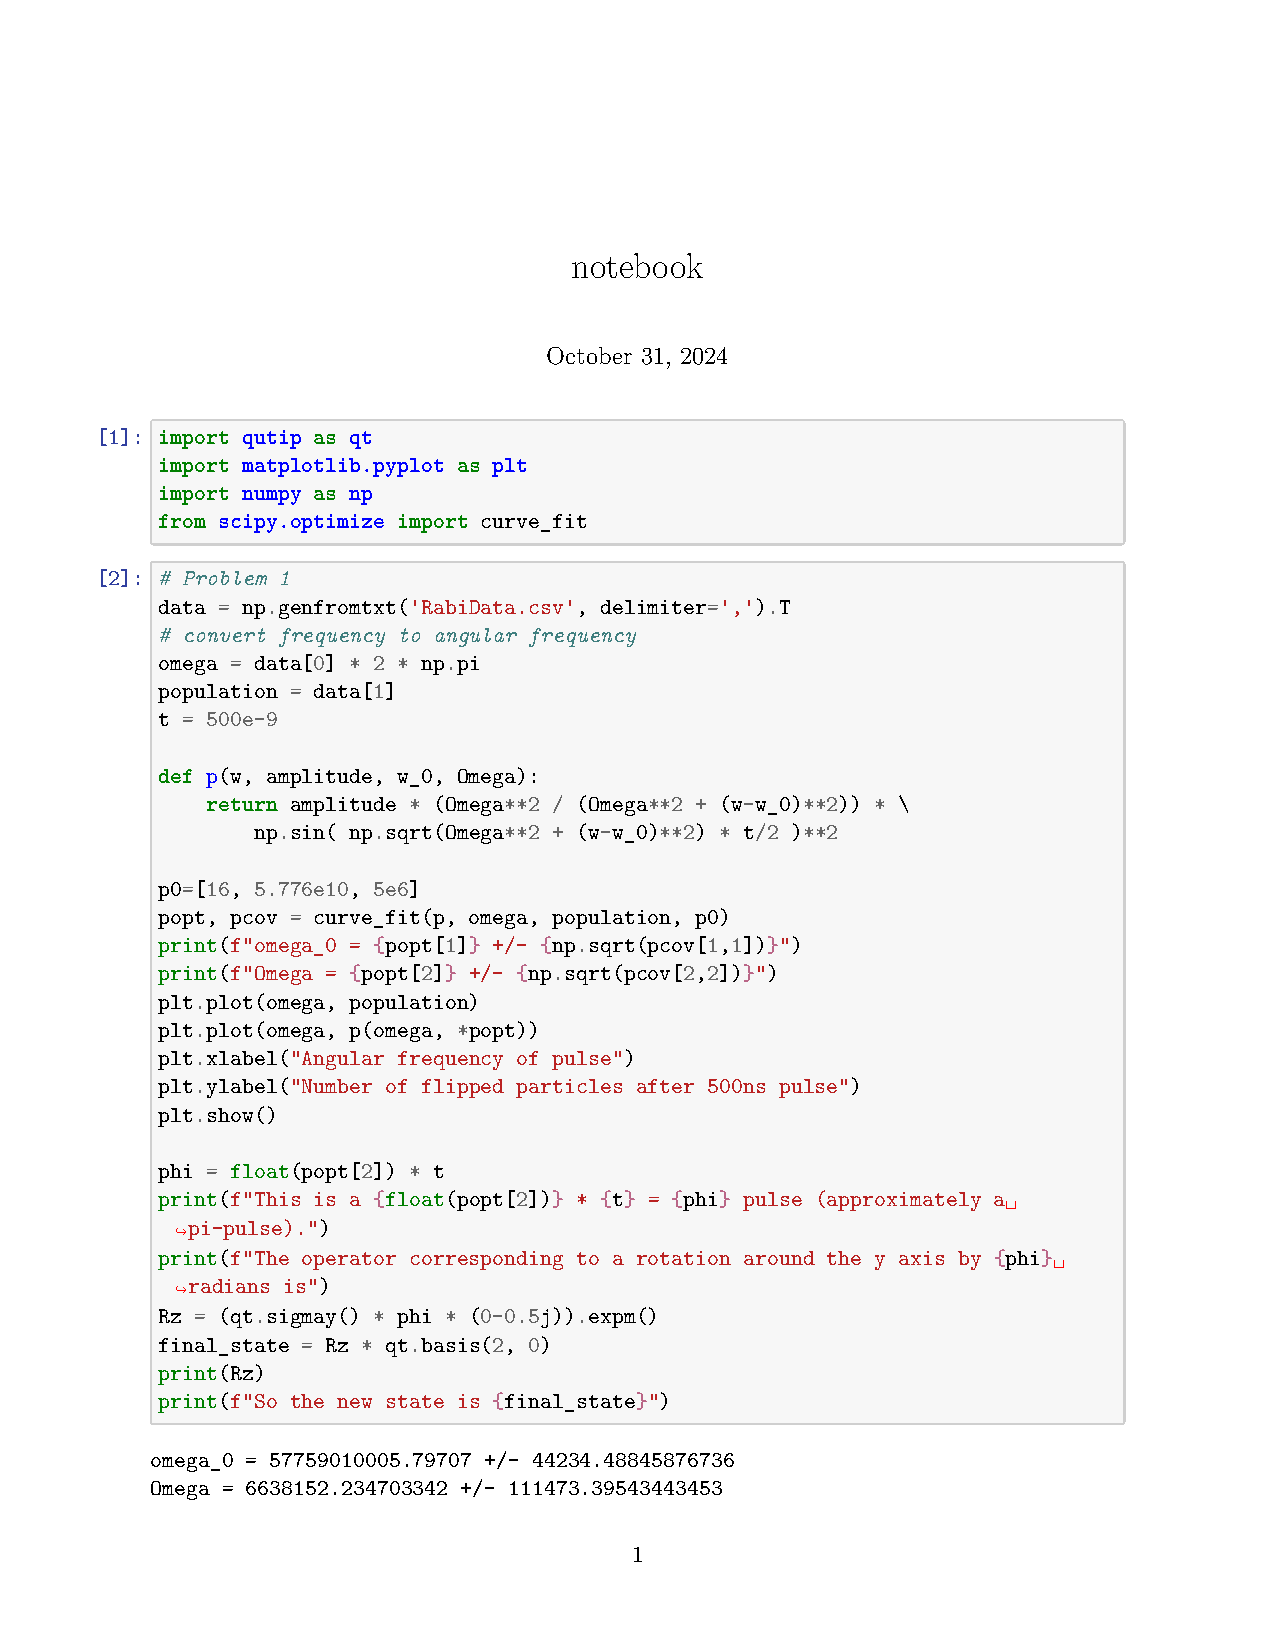
\includepdf[pages=-]{notebook.pdf}
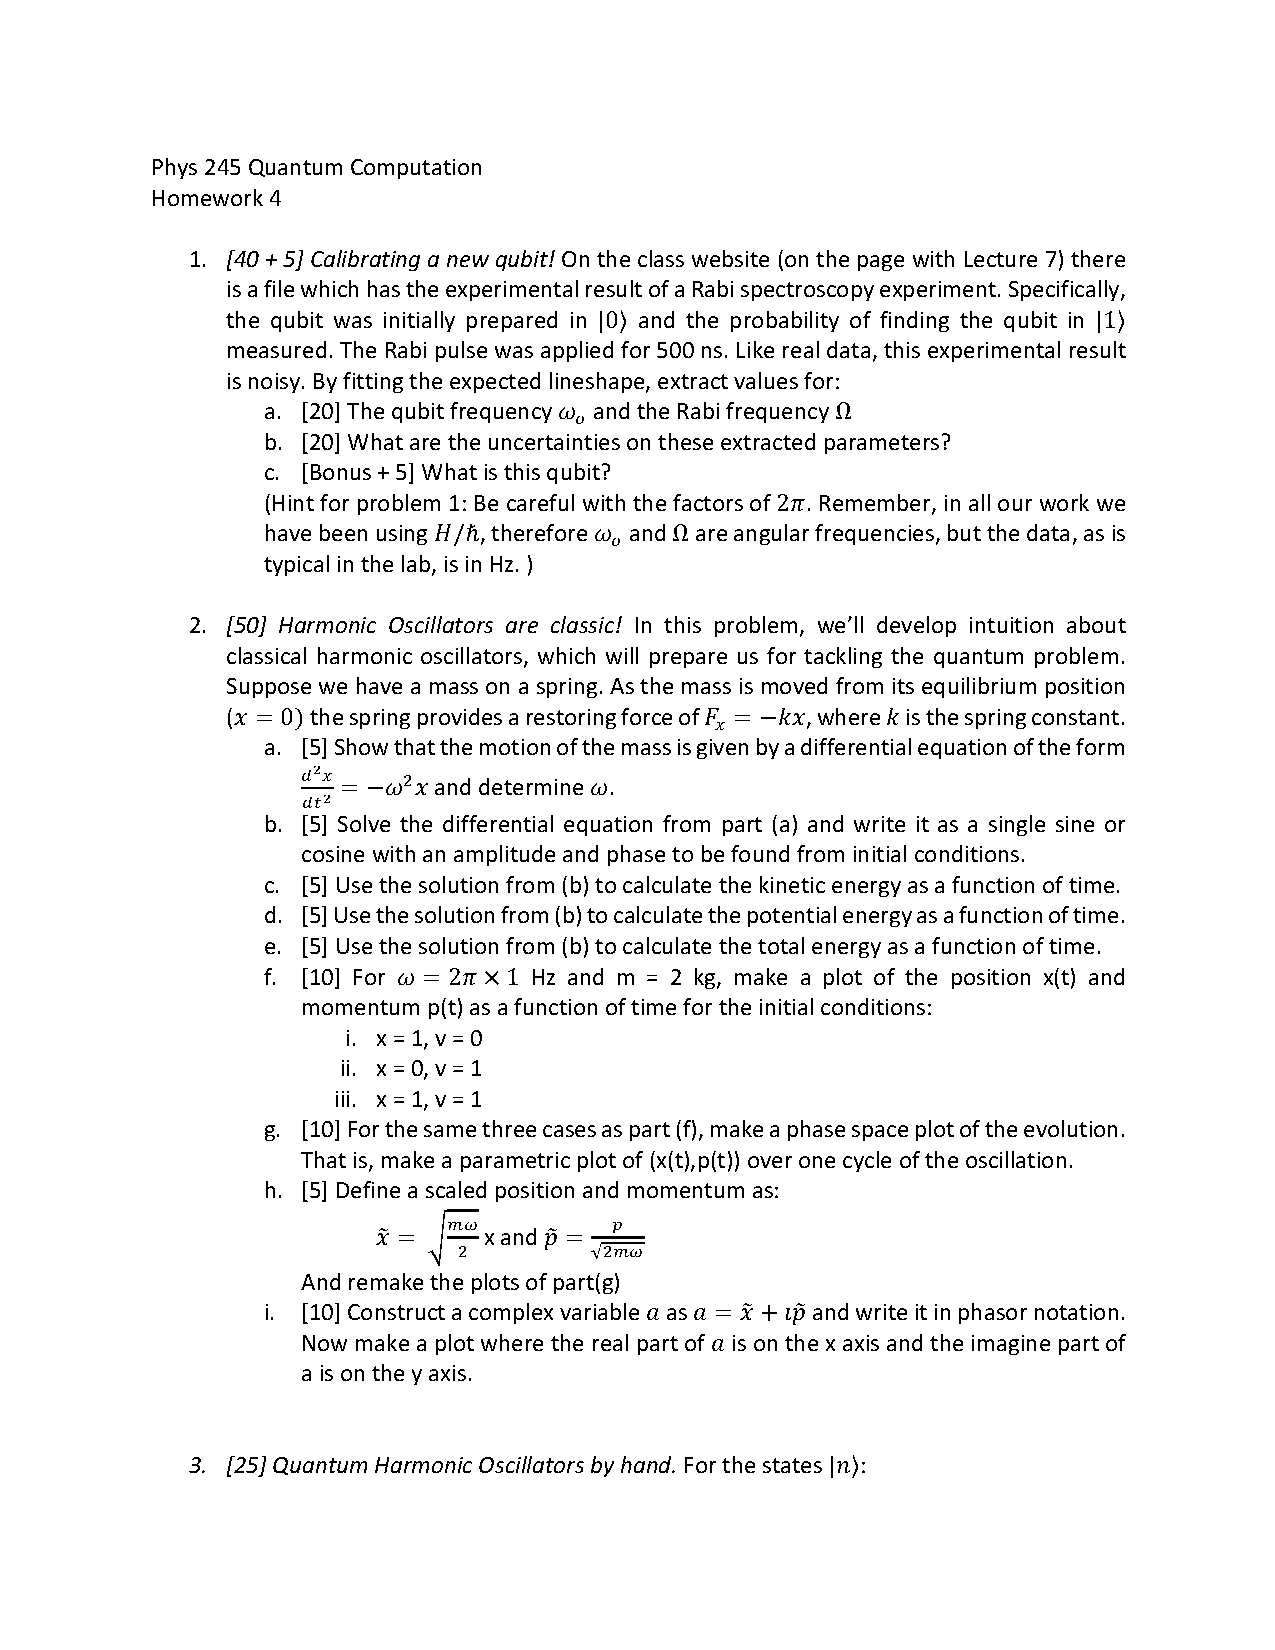
\includepdf[pages=-]{assignment.pdf}

\end{document}
